\clearpage 
\section*{Domande di esame per il capitolo}%
\begin{quest}[Da che principio deriva Dulong-Depetit?]{quest:Da che principio deriva Dulong-Depetit?}
Equipartizione della energia.
\end{quest}
\begin{quest}[Perché $C_v$ non raggiunge il limite di Doulong-Depetit nel caso di corpo nero?]{quest:Perché $C_v$ non raggiunge il limite di Doulong-Depetit nel caso di corpo nero?}
    I fotoni non sono limitati in energia, hanno una densità di energia che aumenta con la frequenza. 
    I fononi invece seguono una densità di energia quadratica con la frequenza soltanto per frequenze inferiori alla $\Omega_D$ (frequenza di Debye).\\
    Di conseguenza per i fotoni $C_V\propto T^3$ sempre, mentre per i fononi vale solo in regime di $T<\theta_D$. Fisicamente si ha che per ogni temperatura i fotoni possono avere dei modi con energia maggiore di $kT$ permettendo quindi loro di essere sempre fuori dal regime classico.
\end{quest}
\begin{quest}[Descrivere la distribuzione di energia del corpo nero]{quest:Descrivere la distribuzione di energia del corpo nero}
Importante sapere la forma, il modo in cui cambia al variare della temperatura sia in frequenza che in lunghezza d'onda.\\
L'espressione per tale distribuzione è bene saperla a memoria ma può essere utile anche saperla ricavare (è necessario saper ricavare la $\rho(\omega)$ per il corpo nero), viene chiesta spesso.
\end{quest}
\begin{quest}[Dove si trova il massimo della distrib. di corpo nero?]{quest:Dove si trova il massimo della distrib. di corpo nero?}
Legge di spostamento di Wien:
\[
    \omega_{\text{max}} \propto T
.\] 
\end{quest}
\begin{quest}[Come osservare la radiazione di corpo nero della stanza in cui ti trovi?]{quest:Come osservare la radiazione di corpo nero della stanza in cui ti trovi?}
    Spegnere le luci e sbarrare tutto, è necessario fornirsi di un sensore infrarossi ($\lambda\sim 10 \mu$m) 
\end{quest}
\begin{quest}[Ricavare la distribuzione di energia del corpo nero]{quest:Ricavare la distribuzione di energia del corpo nero}
    É necessario ricavare $\rho (\omega) d\omega$ e successivamente scrivere $u(\omega) d\omega  = \rho (\omega) \overline{n}\hbar \omega$. Ricordando che la $\overline{n} $ è il numero medio di occupazione degli stati nel caso di Fononi (Bose-Einstein senza $\mu$).
\end{quest}
\begin{quest}[Da dove prende il nome la dist. di corpo nero?]{quest:Da dove prende il nome la dist. di corpo nero?}
    Abbiamo un corpo perfettamente in equilibrio con la radiazione elettromagnetica che contiene, questo significa che può essere considerato perfettamente assorbente a tutte le frequenze e quindi corpo nero. 
\end{quest}
\begin{quest}[Parlare della conducibilità elettrica dei metalli]{quest:Parlare della conducibilità elettrica dei metalli}
    Applicare l'equazione del trasporto di Boltzmann, approssimare $f\approx f_0$ nelle derivate della equazione ed utilizzare la distribuzione di Fermi a gradino. Ne risulterà che la $f$ cambia come $\delta (\mathcal{E}-\mu_F)$ e che quindi gli unici elettroni disponibili alla conduzione sono quelli aventi energia in un intorno $kT$ dell'energia di Fermi.
\end{quest}
\begin{quest}[Perché la $\rho$ nel caso di corpo nero si accorge della forma delle pareti?]{quest:Perché la  nel caso di corpo nero si accorge della forma delle pareti?}
Perché per ricavarla è necessario imporre delle condizioni al contorno che tengono appunto di conto delle pareti. 
\end{quest}

\begin{quest}[Quale tra i seguenti due materiali conduce meglio? (immagini) ]{quest:Quale tra i seguenti due materiali conduce meglio? (immagini) }
\begin{figure}[H]
    \centering
    \incfig{chi-conduce-meglio?}
    \caption{chi conduce meglio?}
    \label{fig:chi-conduce-meglio?}
\end{figure}
Ci sono due contributi alla conducibilità in questo caso: 
\begin{itemize}
    \item La concavità della parabola (più ripida è la conca e minore è la massa efficace)
    \item Il numero di elettroni che è maggiore nel caso di parabola più schiacciata.
\end{itemize}
È necessario capire se vince la quantità di elettroni oppure il fatto che con massa efficace minore ne accelero di più. 
Per rispondere è necessario ricordare il coefficiente $\sigma$ per la conducibilità:
\[
    \sigma  = \frac{e^2n}{m}\tau (\mu_F) 
.\] 
Dove si ricorda che $J = \sigma E$. Nei due casi abbiamo due masse diverse, dobbiamo giocarcela con gli $n$ (diversi anche quelli) per capire chi conduce di più.
Per trovare $n$ possiamo vedere chi dei due ha più elettroni: 
\[
    N = \int_{0}^{\mathcal{E}_F} \rho (\mathcal{E}) d\mathcal{E}\propto\left(\mathcal{E}_F\cdot m\right)^{3 /2} \implies  n = \frac{N}{V}
.\] 
In conclusione abbiamo che:
\[
    \frac{\sigma_1}{\sigma_2} = \frac{m_1^{1 /2}}{m_2^{1 /2}}
.\] 
Supponiamo che $m_1>m_2$, in tal caso si ha $\sigma_1>\sigma_2$, quindi vince la parabola più schiacciata.	
\end{quest}

\begin{quest}[É possibile fare condensaz. di BE con i fotoni?]{quest:É possibile fare condensaz. di BE con i fotoni?}
    Il problema con i fotoni è che non conservano il numero di particelle, quindi quanto tento di raffreddare il sistema (facendo $\mu\to 0$ e $N\to \infty$ nel caso di particelle Bosoniche (ATTENZIONE CHE QUI $\mu$ NON C'È PER I FOTONI)) non c'è nessun problema con il fatto che $N$ non diverga: i fotoni semplicemente spariscono!\\
    È quindi necessario trovare un modo per conservare il numero di fotoni. Nel caso di corpo nero non c'è modo di far questo: il numero di fotoni tende a zero. 
    Si deve prendere un sistema in grado di riemettere lo stesso numero di fotoni che assorbe. Nella pratica si costruisce una "scatola" che funzioni come un sistema a due livelli (all'orale si è parlato di una scatola di oscillat. armonici), tale sistema insieme a dei fotoni termalizzati con un range di energia molto stretto può permettere la condensazione.
\end{quest}
\begin{quest}[Parlare della condensazione di Bose-Einstein]{quest:Parlare della condensazione di Bose-Einstein}
Forma della distribuzione e espressione della distribuzione da dire al volo. Calcolare il numero medio di particelle e spiegare perché non diverge\ldots Argomentare.
\end{quest}
\begin{quest}[Perché le particelle nel fondamentale non vengono considerate nella $\rho$?]{quest:Perché le particelle nel fondamentale non vengono considerate nella $rho$?}
Non avendo energia lo stato fondamentale, secondo la nostra $\rho \propto  \mathcal{E}^{1 /2}$, ha densità di stati nulla.
\end{quest}
\begin{quest}[Esiste sistema per il quale $N\to \infty$ con $\mu\to 0$ nel caso di Bosoni?]{quest:Esiste sistema per il quale $Ntoinfty$ con  nel caso di Bosoni?}
    Si, basta prendere un sistema 2D, in tal caso la densità di stati è indipendente dall'energia e l'integrale della (sola) Bose-Einstein da 0 a $\infty$ può divergere: in 2 dimensioni niente condensato =(
\end{quest}

\begin{quest}[Calore specifico per il gas di Bosoni]{quest:Calore specifico per il gas di Bosoni}
    In regime classico tornerà $C_V = 3 /2 NK$. In regime quantistico al di sotto della temperatura critica possiamo approssimare $\mu\approx  0$ procedere al calcolo della energia:
\[
    E \propto  \int_0^{\infty} \overline{n}\mathcal{E}^{1 /2}\cdot \mathcal{E}  d\mathcal{E}
.\] 
Con il classico cambio di variabile $x = \mathcal{E}  /kT$ si arriva ad avere:
\[
    E \propto  \left(kT\right)^{5 /2}
.\] 
E quindi $C_V \propto T^{3 /2}$. Nel regime intermedio il calore specifico presenterà una sorta di overshoot da questo andamento che lo porta a salire leggermente al di sopra del calore specifico di Doulong-Depetit poiché $C_V(T_c) \approx 1.9 NK > 1.5 NK$.
\end{quest}
\begin{quest}[Parlare dell'effetto fotoelettrico]{quest:Parlare dell'effetto fotoelettrico}
\end{quest}
\begin{quest}[Come va il calore specifico per un foglio di grafite?]{quest:Come va il calore specifico per un foglio di grafite?}
In due dimensioni abbiamo che ad alte temperature torna l'andamento $3Nk$, a basse temperature non abbiamo l'andamento $T^2$ come invece ci si aspetterebbe: il sistema è immerso in un um mondo 3D e tutti i 3 modi vibrazionali sono ancora accessibili.
\end{quest}
\begin{quest}[Data la dispersione del grafene rispondere alle domande in descrizione]{quest:Data la dispersione del grafene indicare quali modi sono sul piano}
    \begin{figure}[H]
        \centering
	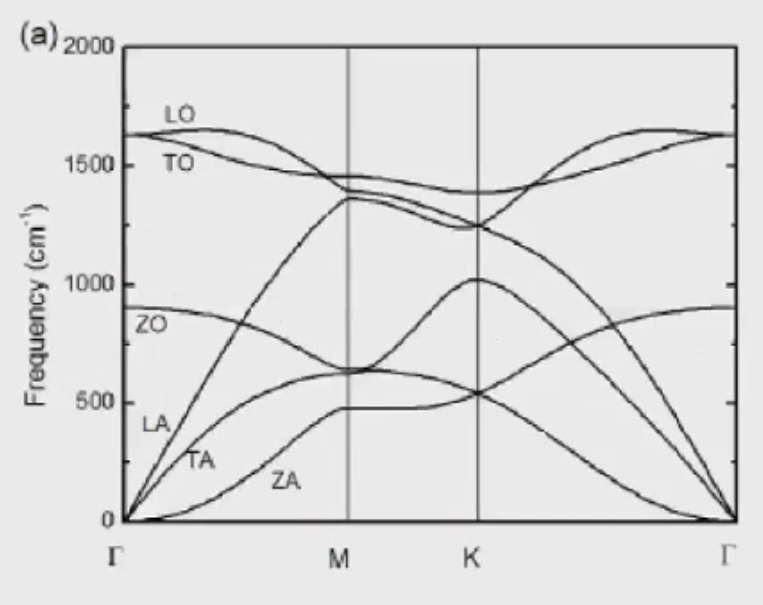
\includegraphics[width=0.4\textwidth]{figures/dipersione_grafene.png}
        \caption{Curve di dispersione del grafene: qual'è la banda che indica i moti nel piano? Perché?}
        \label{fig:figures-dipersione_grafene-png}
    \end{figure}
    La banda meno energetica è quella che si muove nel piano, quindi la ZA. Questo è spiegato dal fatto che fuori dal piano non ci si avvicina a nessun altro atomo, quindi il moto è meno energetico. É più facile piegare un foglio in direzione ortogonale al foglio rispetto a farlo scorrere nel piano stesso.
\end{quest}
\begin{quest}[Dal grafico \ref{fig:figures-dipersione_grafene-png} possiamo dedurre l'andamento di $C_v$ per il grafene a basse $T$?]{quest:Nel grafico di figura}
Una delle tre curve ha una dispersione parabolica anziché lineare:
\[
    \mathcal{E}\propto k^2  \propto  p^2
.\] 
Quindi abbiamo anche che 
\[
    p \propto  \sqrt{\mathcal{E}} 
.\] 
Conteggiando gli stati ottengo il risultato che otterrei per un sistema bidimensionale:
\[
    \rho (\mathcal{E}) = \text{cost}
.\] 
Quindi anche $C_v\propto T$. Un altro calore specifico che va linearmente come la temperatura è quello del gas di elettroni in un cristallo!
\end{quest}
\begin{quest}[Nel grafico \ref{fig:figures-dipersione_grafene-png} i fononi ottici long. e trasv. sono isoenergetici a $k=0$, perché?]{quest:Nel grafico i fononi ottici long. e trasv. sono isoenergetici a $k=0$, perché?}
    I fononi ottici longitudinali trasportano un campo elettrico macroscopico, per questo non dovrebbero essere uguali nell'origine. Il grafene non ha un momento dipolare nella cella unitaria (c'è solo il carbonio), quindi nessun campo elettrico.
\end{quest}
\begin{quest}[Nel grafico \ref{fig:figures-dipersione_grafene-png} come si spiegano le degen. in $M$?]{quest:Nel }
Tali degenerazioni sono date da particolari simmetrie nel cristallo, questo perché nel punto di contatto si può estendere la zona di Brillouin: c'é una simmetria più alta rispetto al resto della zona. Praticamente è come dire che in quella direzione vedo una catena di atomi equispaziati.
\end{quest}
\begin{quest}[In un gas di fermioni è tanto importante la densità di stati per il calcolo di $C_V$?]{quest:In un gas di fermioni è tanto importante la densità di stati per il calcolo di $C_V$?}
Nel caso di distribuzione di Fermi abbiamo che solitamente è possibile approssimare a gradino, quindi in questo caso la forma funzionale della densità di stati non conta molto, contano soltanto gli elettroni aventi energia $\mathcal{E}_F$. 
Nella Bose-Einstein contano essenzialmente quelli con $\mathcal{E} =0$. Quindi per i Fermioni la dipendenza dall'energia è congelata (diventa $\mathcal{E}_F$) nel caso di Bosoni invece la dipendenza è pesante.
\end{quest}

